\section{TASARIM}

\subsection{Genel Bilgiler}

Projenin tasarımı kapı eşiklerinde kullanılmaya uygun olacak şekilde düşünülmüştür. Temel amaç kapı eşiğinden bir kişi geçtiğinde kişi ile ilgili LDR'den gelen voltaj verilerini toplamaya dayalıdır. Bir Bluetooth modülü, bir harici güç kaynağı, bir STM32H723ZG mikroişlemci kartı ve iki adet LDR sensöründen oluşmakta olan sistem bir kutu şeklinde duvara veyahut kapı eşiklerine monte edilebilecek şekilde tasarlanmıştır. \ref{fig:mickutu}de sistemin kutusu görülmektedir.


\begin{figure}[H]
    \centering
    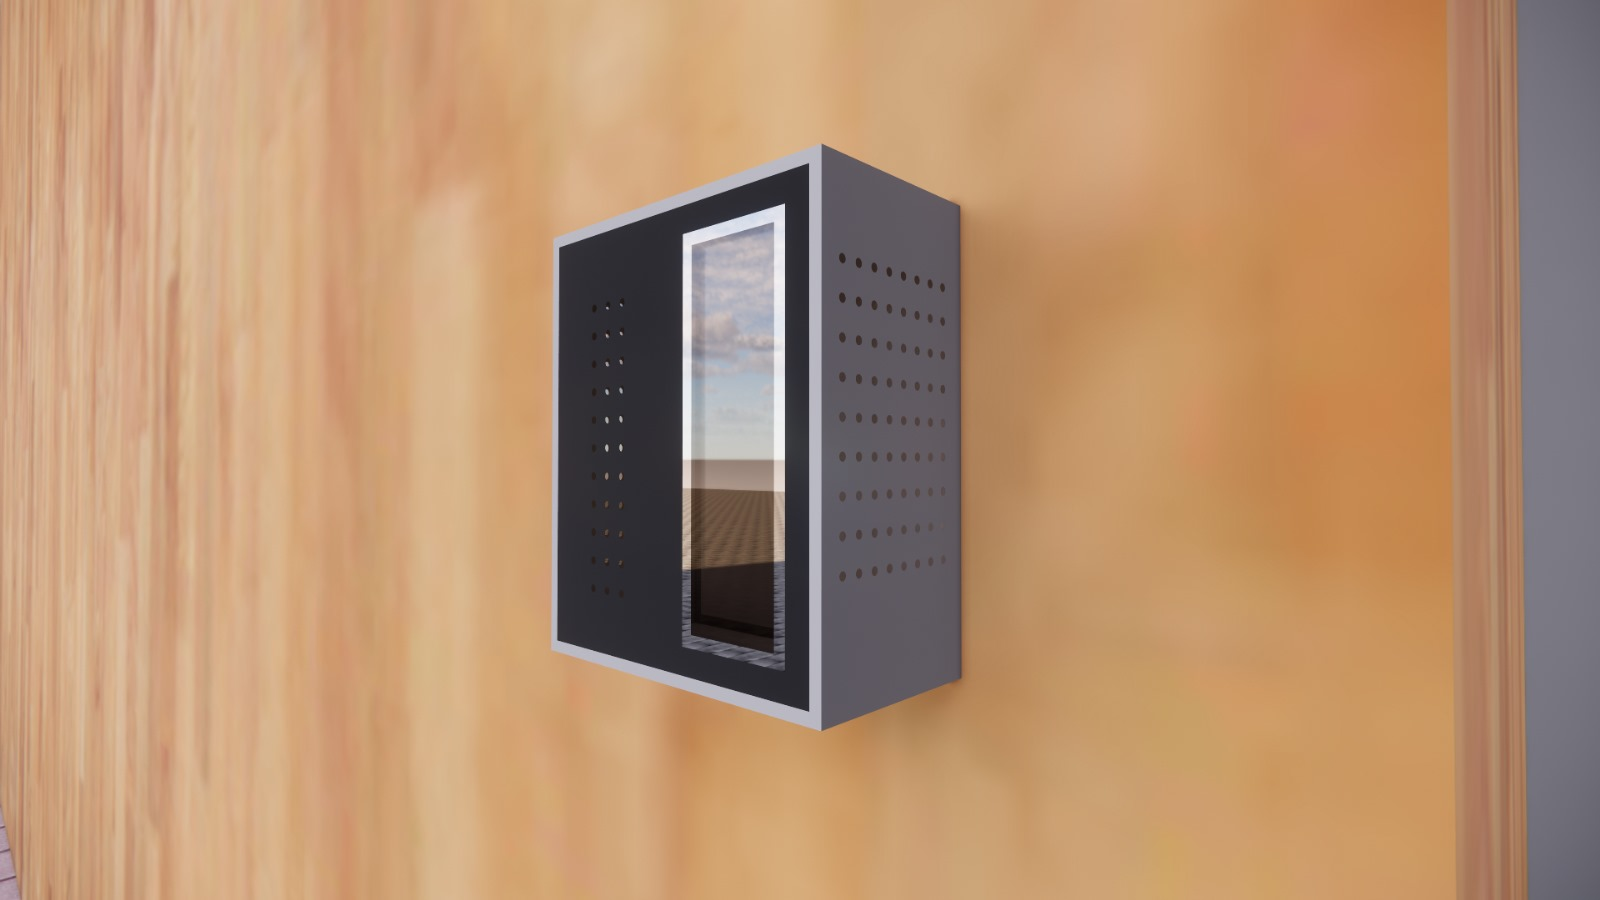
\includegraphics[width=\linewidth]{image14}
    \caption{Sistemin Kutusu}
    \label{fig:mickutu}
\end{figure}


Projenin tasarımında en önemli husus, ışık temelli algılama yapılması nedeniyle sistemin kullanılacağı ortamların yeterli düzeyde ışıklandırmaya sahip olması gerekliliğidir. Bu amaçla projede iki adet LDR (Light Dependent Resistor) sensörü kullanılmıştır. Kişinin hareket hızının tespiti istendiğinde, en az iki sensör gerekmektedir; böylece birinci sensör ile ikinci sensör arasında geçen süre ölçülerek hız hesabı yapılabilir.

Sistem, harici bir güç kaynağı ile beslenmektedir. Bu güç kaynağı, olası enerji kesintilerinde sistemin ani şekilde kapanmasını engellemektedir ve modüler kullanım imkânı sağlamaktadır. Verilerin bilgisayara aktarılması için Bluetooth modülü kullanılmıştır. Bluetooth modülü, mikrodenetleyici ile bilgisayar arasında kablosuz haberleşmeyi sağlamaktadır.

Başlangıçta projede MSP430 mikrodenetleyici kartı tercih edilmiştir. MSP430'un haberleşme portlarına Bluetooth modülünün doğrudan entegre edilebilmesi, üzerinde kolaylıkla elektronik devreler kurulabilmesi, erişim kolaylığı ve düşük maliyeti bu tercihte etkili olmuştur. Ancak MSP430 mikrodenetleyicisinin işlem gücünün yetersiz kalması ve üzerinde yapay zeka tabanlı bir modelin çalıştırılamaması nedeniyle, daha yüksek performansa sahip olan STM32H723ZG mikrodenetleyicisi projeye entegre edilmiştir. STM32H723ZG, ARM Cortex-M7 mimarisi sayesinde yüksek hesaplama kapasitesi sunmakta ve yapay zeka algoritmalarının çalıştırılmasına olanak tanımaktadır.

Projenin akış diyagramı Şekil \ref{fig:akış}'te, MSP430 işlemcisi aracılığıyla sensörlerden veri almak ve bilgisayar üzerinde yapay zeka modelini oluşturmak amacıyla kurulan elektriksel bağlantılar  ise Şekil \ref{fig:elk_devre}'de gösterilmiştir. Projenin son safhasında modeli koşturan ve verileri dinamik olarak işleyen STM32H723ZG işlemcisinin bağlantı şeması \ref{fig:stmbaglanti}'da  verilmiştir.

\begin{figure}[H]
    \centering
    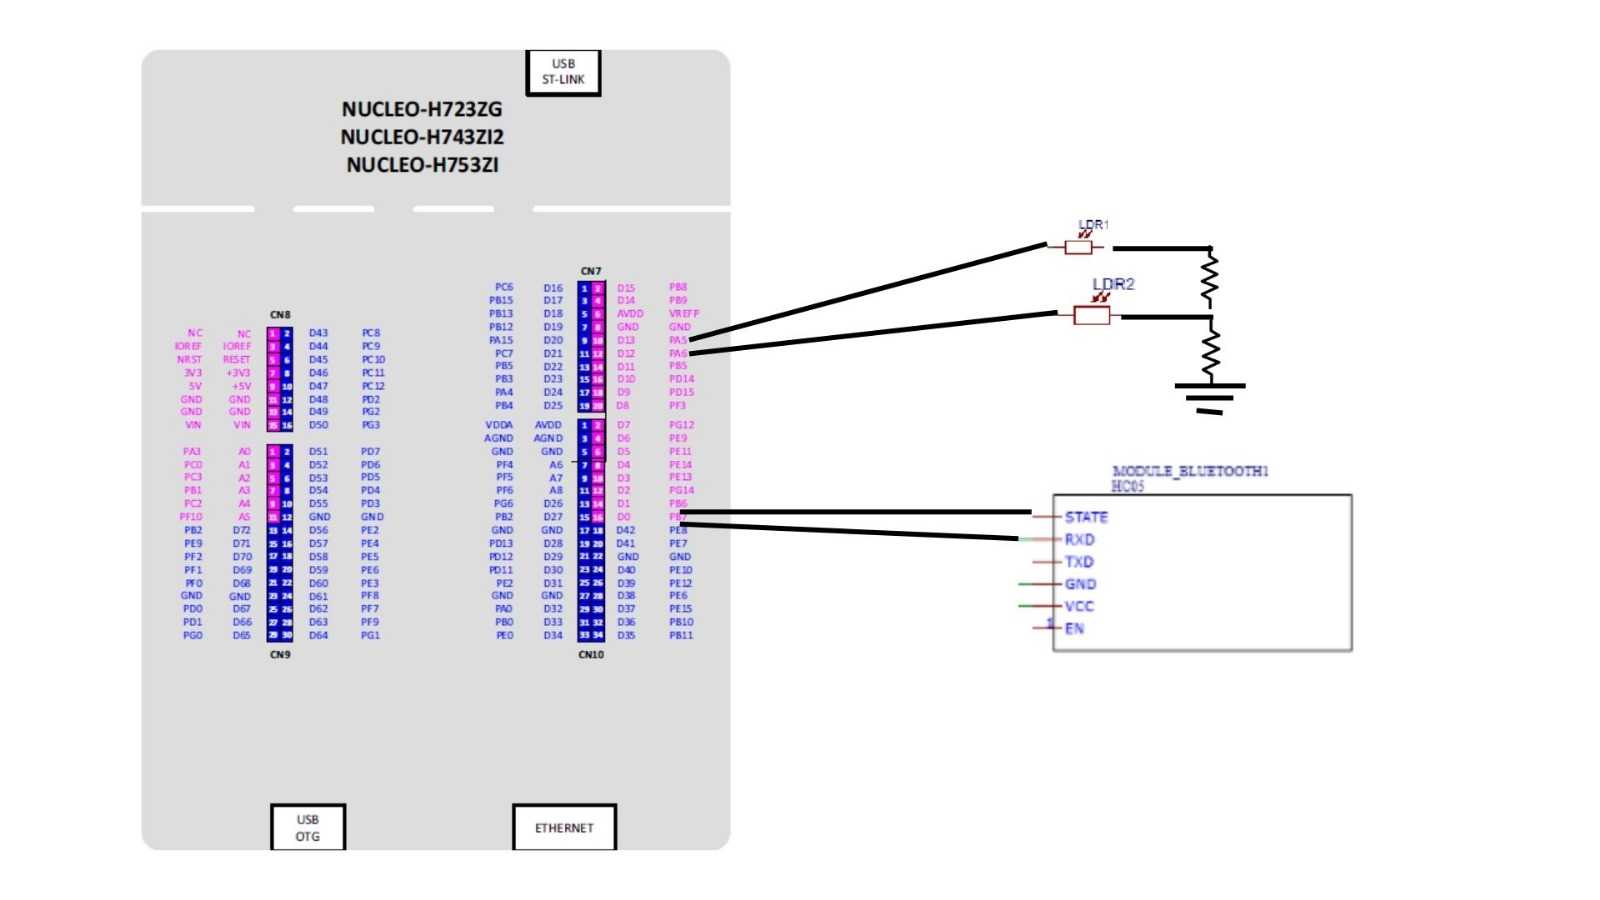
\includegraphics[width=0.75\linewidth]{stmsema.jpg}
    \caption{STM32H723 Bağlantı Şeması}
    \label{fig:stmbaglanti}
\end{figure}

\begin{figure}[H]
    \centering
    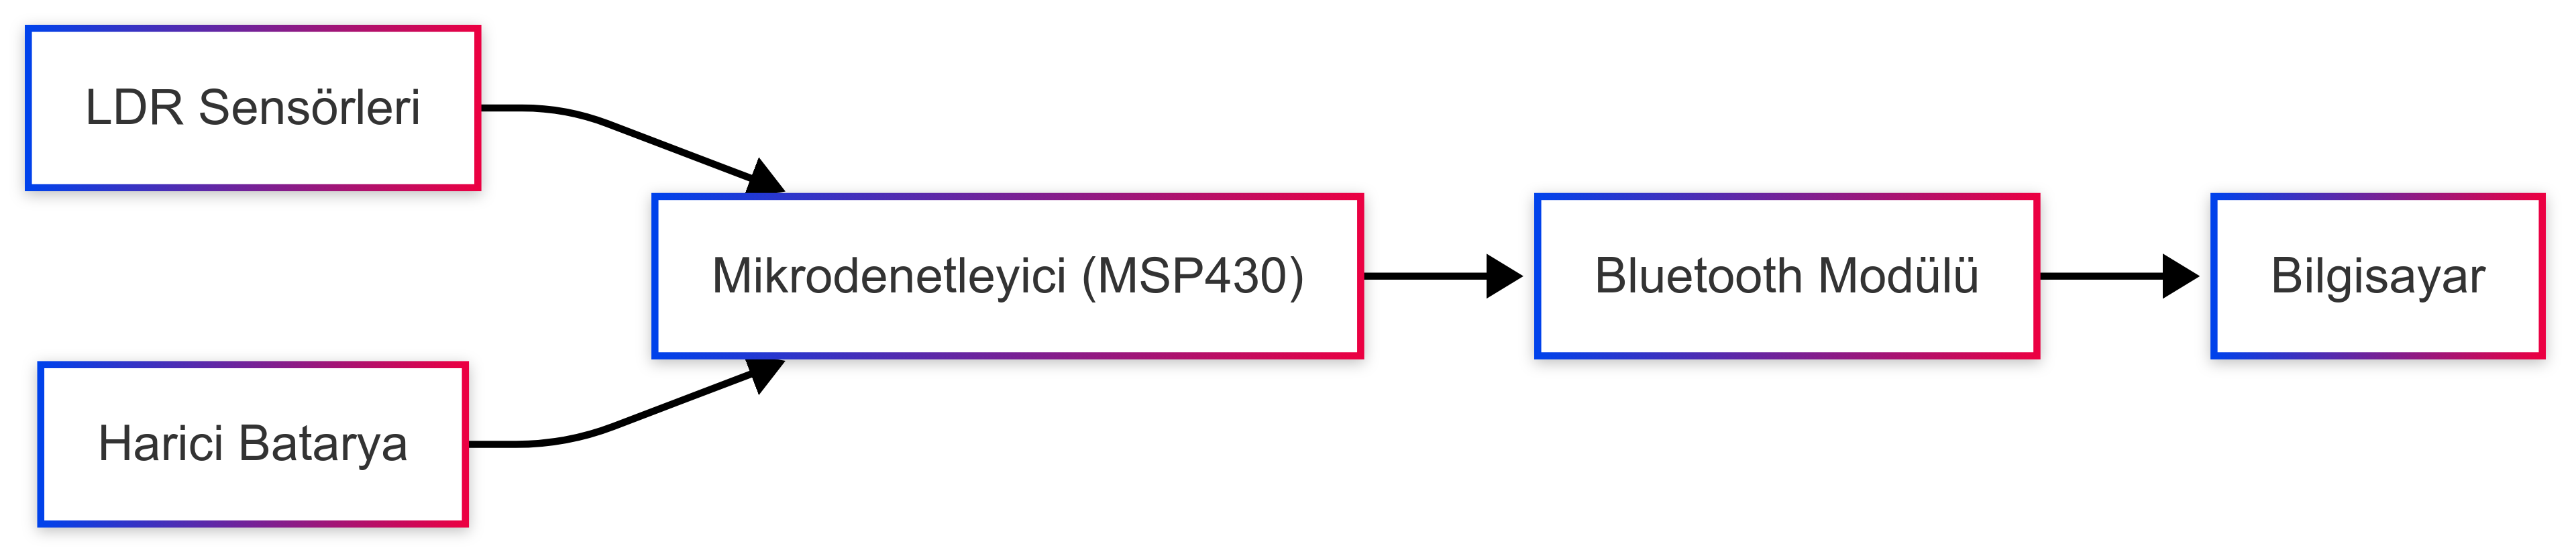
\includegraphics[width=\linewidth]{image12}
    \caption{Veri Toplama Akış Diyagramı}
    \label{fig:akış}
\end{figure}


\subsection{Boyutlandırmalar}

Proje eni 5.8 cm, boyu 8.4 cm, yükekliği 18 cm bir kutu olarak tasarlanmıştır. Kutu proje içerisinde kullanılan tüm bileşenleri kutu içerisine rahatça sığacağı bir hacimdedir; ayrıca içerideki bileşenlerin ısınmaması için havalandırma delikleri ile çözüm üretilmiştir. Havalandırma deliklerinin çapı 0.2 mm'dir. Sensörlerin içine sığacağı yuvaların çapı 0.3 mm'dir. Sensör yuvaları kutunun geçen kişiye bakan ön yüzünde bulunmaktadır. STM32H723ZG kartının boyutları 13.3 cm x 7 cm'dir. HC05 seri Bluetooth modülünün boyutları 35 mm x 15 mm'dir. 

Projenin Karadeniz Teknik Üniversitesi bitirme projeleri sunumlarında gösterilebilmesi amacıyla, harici batarya ile birlikte taşınabilir ve geçici bir tasarım kullanılmıştır. Bu geçici tasarımın boyutları, ana tasarımla yaklaşık olarak aynıdır. Geçici tasarım  \ref{fig:gecici}'de gösterilmiştir.

\begin{figure}[H]
    \centering
    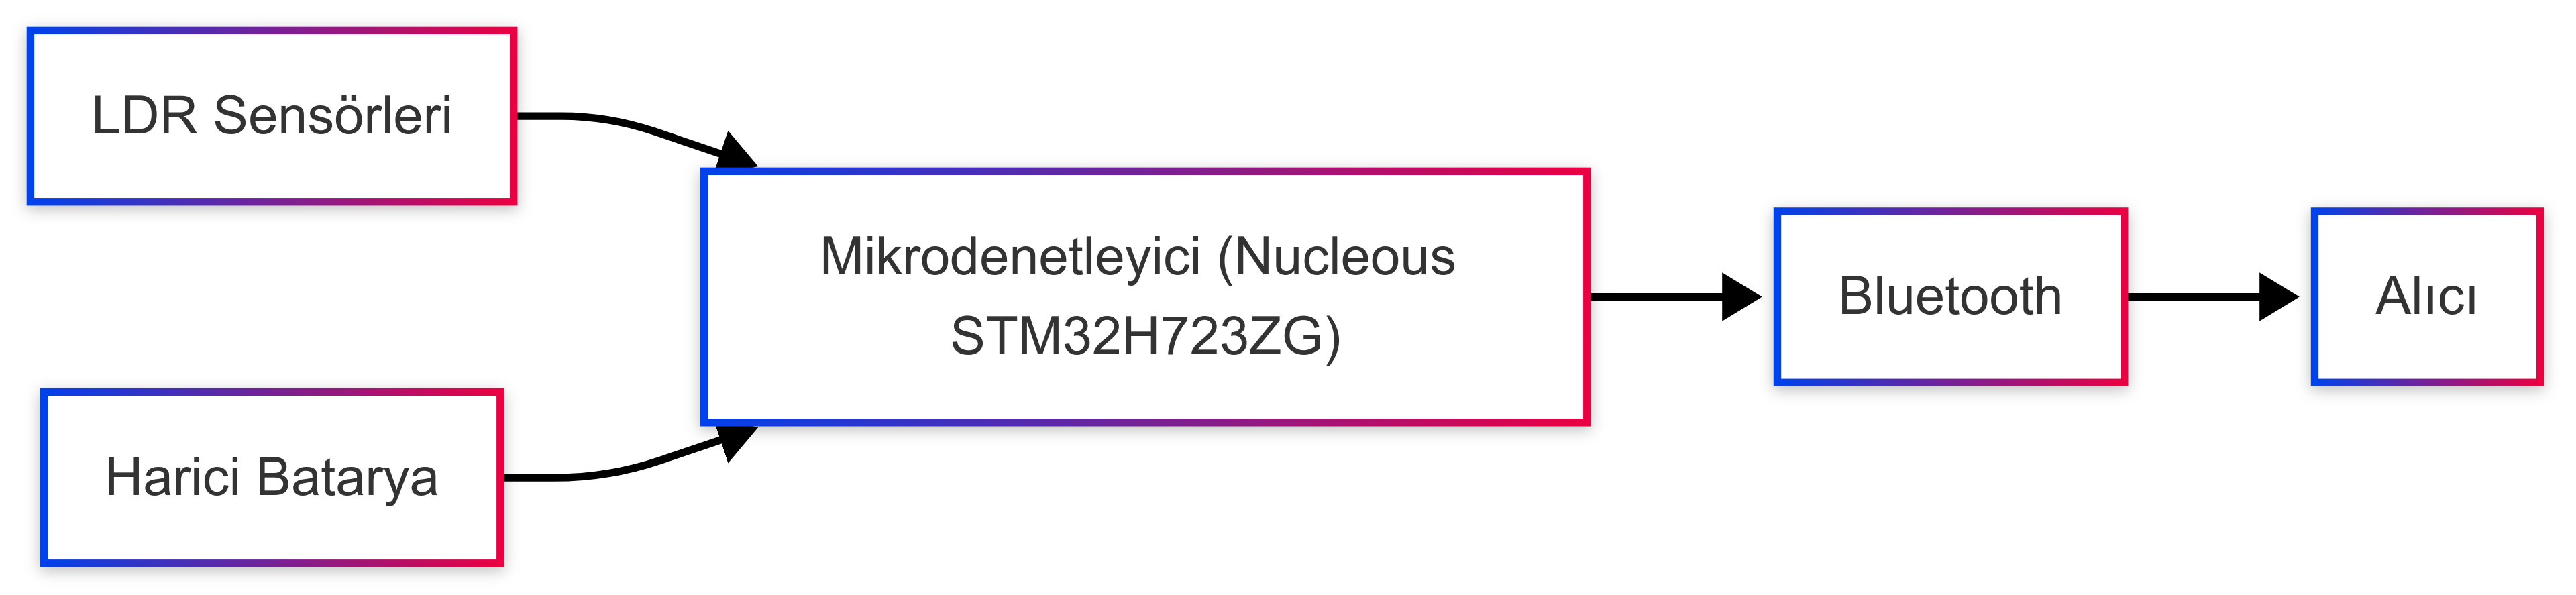
\includegraphics[width=\linewidth]{image12_1}
    \caption{Yapay Zeka Koşturma Akış Diyagramı}
    \label{fig:akış2}
\end{figure}

\begin{figure}[H]
    \centering
    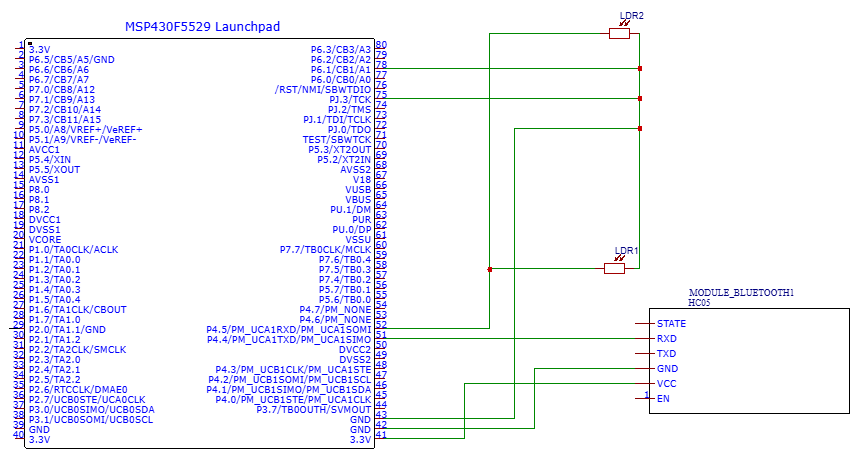
\includegraphics[width=0.8\linewidth]{image18}
    \caption{MSP430 Üzerinde Kurulan Elektrik Devresi}
    \label{fig:elk_devre}
\end{figure}


\subsection{Sistem Bileşenleri ve Seçimleri}

\subsubsection{MSP430F5529LP}
MSP430 Mikrokontrolcü Texas Instruments tarafından geliştirilen bir platformdur. Kendi 16-bit RISC(Reduced Instruction Set Computer) mimarisini kullanan mikrokontrolcünün düşük güç tüketimi ile verimli çalışma kapasitesi dolayısıyla sistemin harici batarya ile çalışma süresini uzatması, içerisinde bulunan 12 bitlik ADC ile voltajların dijital sinyale dönüşümünü dahili olarak gerçekleştirebilmesi, üzerine Bluetooth modülü entegre edilebilmesi tercihindeki ana unsurlar olmuştur. \ref{fig:MSP_HC05}de MSP430 mikrodenetleyicisi görülmektedir.

\begin{figure}[H]
    \centering
    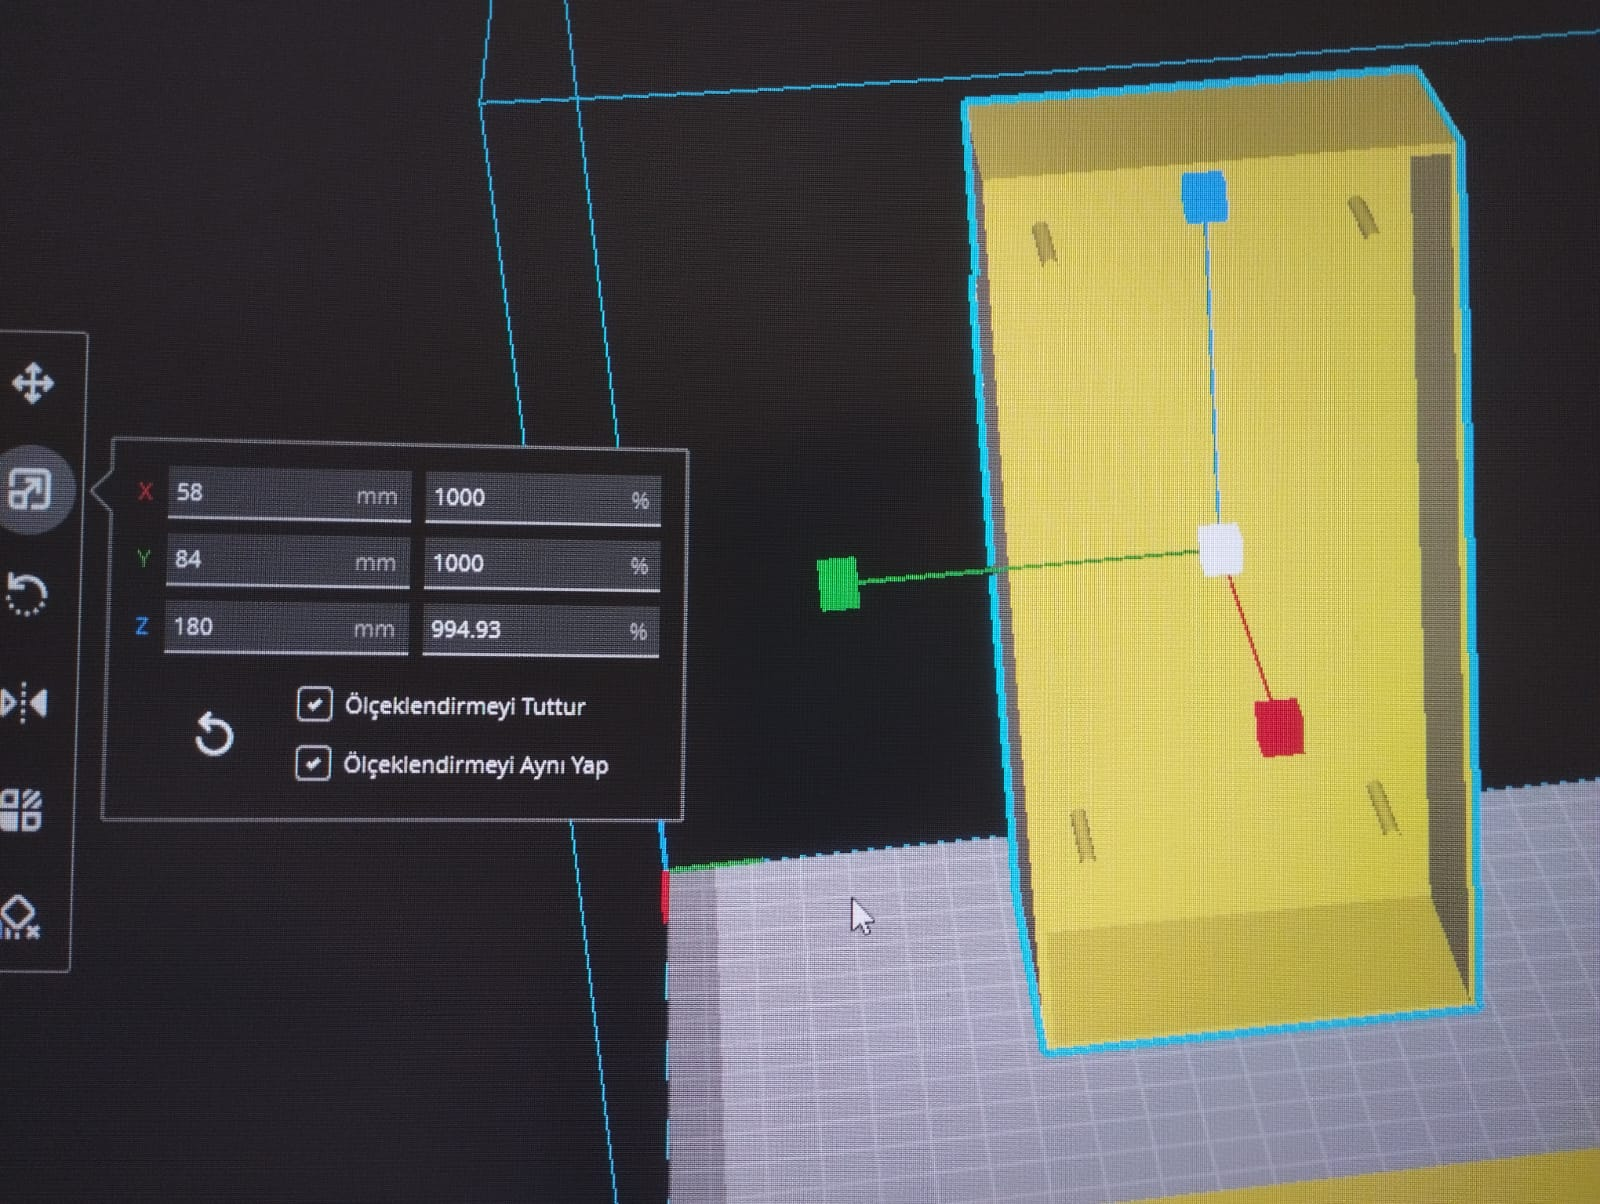
\includegraphics[width=0.75\linewidth]{kutu.jpg}
    \caption{Geçici Tasarım}
    \label{fig:gecici}
\end{figure}

\subsubsection{HC05 Seri Bluetooth Modülü}
HC-05 seri Bluetooth modülü, Bluetooth 2.0 desteği sunan bir entegredir. 10 metreye kadar Bluetooth ile haberleşebilmeyi sağlar. EDR (Enhanced Data Rate) desteği sağlayan entegre, daha hızlı veri aktarımına olanak sağlar. UART haberleşme desteği sağlaması ve 3.3V besleme seviyesinde çalışması, mikrokontrolcü ile uyumunu sağlar. \ref{fig:MSP_HC05}de Bluetooth modülü görülmektedir.

\begin{figure}[H]
    \centering
    % First figure
    \begin{subfigure}{0.45\textwidth}
        \centering
        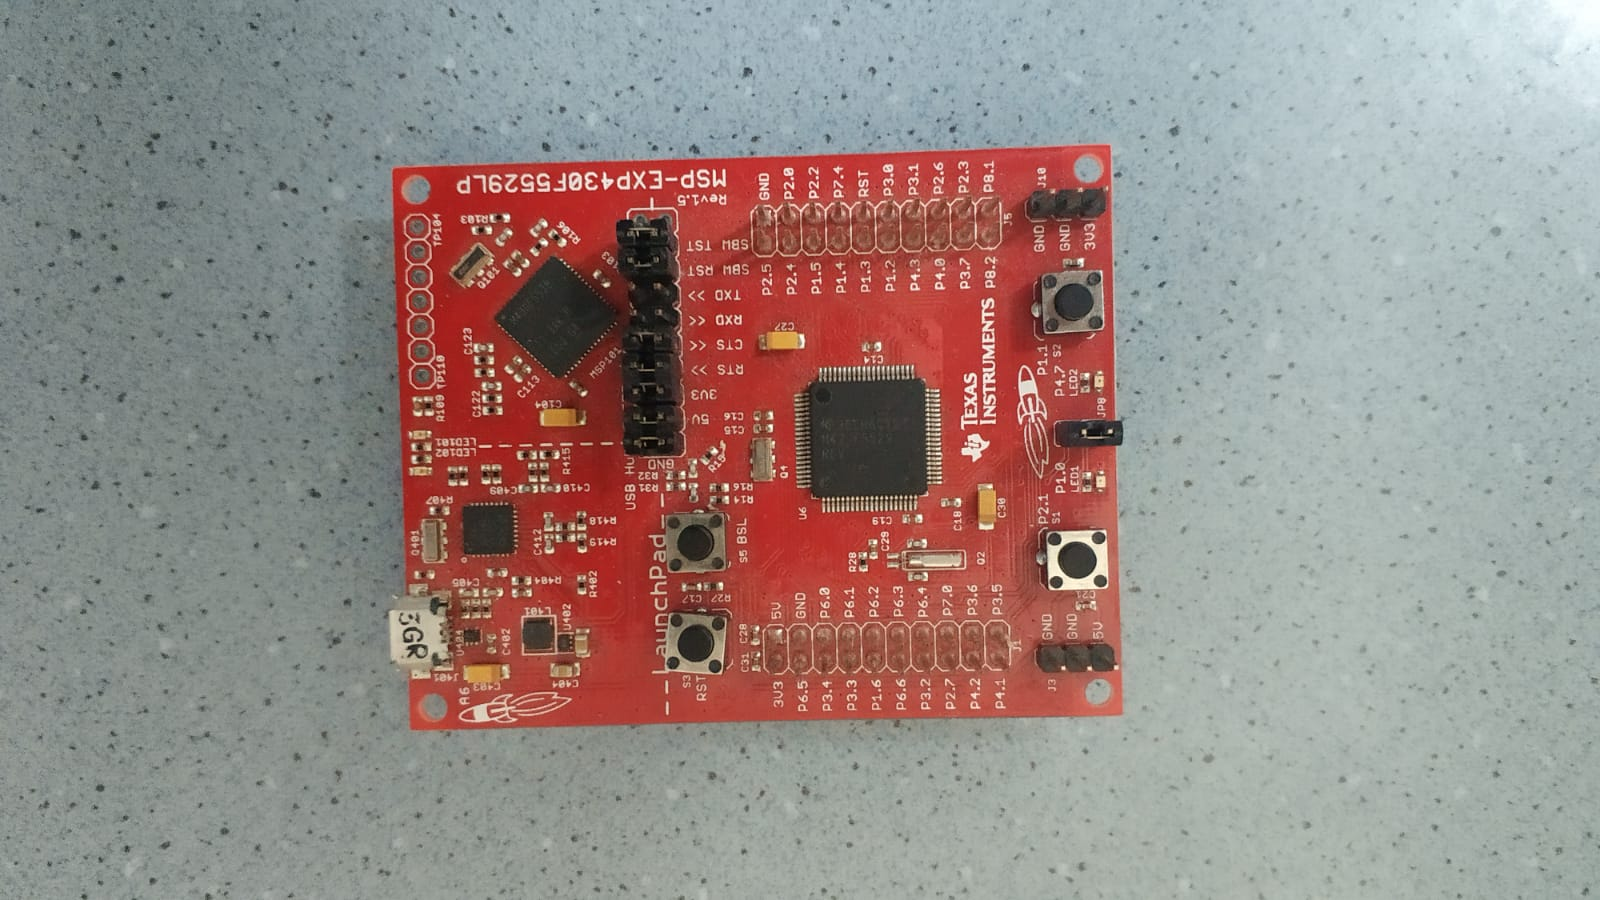
\includegraphics[angle=180, width=\textwidth]{image4x} % Replace with 
    \end{subfigure}
    \hfill
    % Second figure
    \begin{subfigure}{0.45\textwidth}
        \centering
        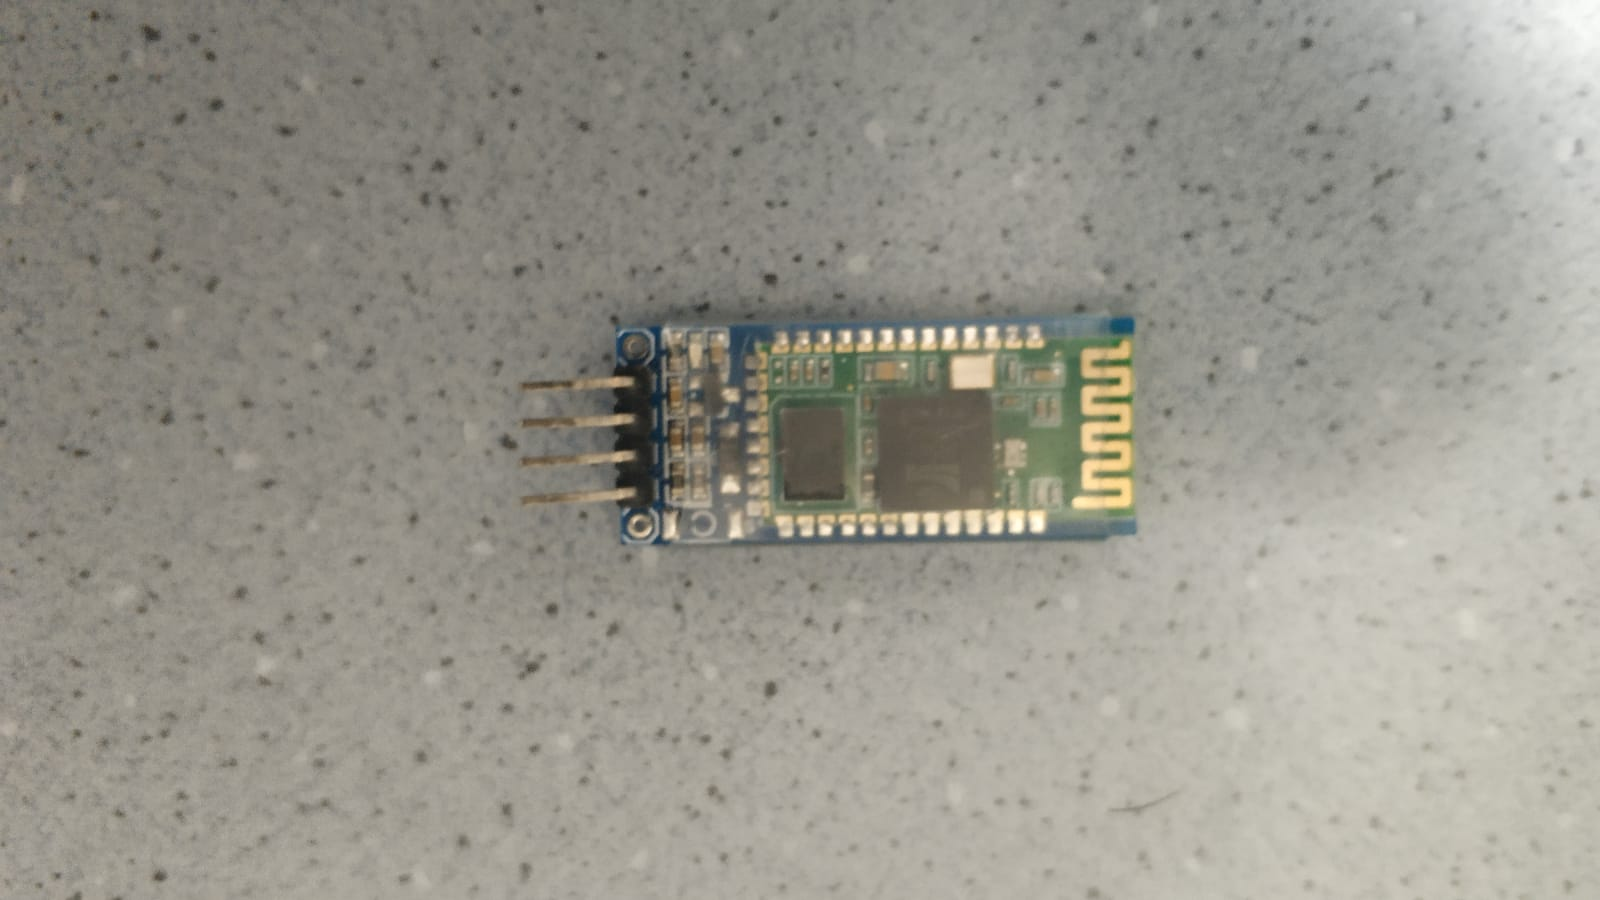
\includegraphics[angle=180, width=\textwidth]{image3x} % Replace with your file name
    \end{subfigure}
    \caption{MSP430F5529LP Mikrodenetleyicisi ve HC05 Seri Bluetooth Modülü}
    \label{fig:MSP_HC05}
\end{figure}



\subsubsection{LDR}

LDR (Light Dependent Resistor), ışığa duyarlı bir dirençtir. Bu bileşenin direnci, üzerine düşen ışık miktarına göre değişir. Ucuz maliyetli bir parçadır. Kutu önünden geçen kişinin ayrımını yapmak için kullanılan voltaj verilerinin elde edilmesi için kullanılır. \ref{fig:pow_ldr}de LDR görünmektedir.



\subsubsection{Harici Güç Kaynağı}
Harici Güç Kaynağı, bir enerji depolama cihazıdır. Projede lityum iyon bataryalı, 10.000 mAh kapasiteye sahip bir harici güç kaynağı kullanılmaktadır. Projenin Karadeniz Teknik Üniversitesi’ndeki sunumlarında, taşınabilirlik ve kesintisiz enerji sağlamak amacıyla sabit güç kaynakları yerine kolay taşınabilir, batarya destekli bir enerji kaynağı tercih edilmiştir. Böylece, sunum sırasında projenin kablo veya priz bağlantısına ihtiyaç duymadan her ortamda rahatlıkla çalıştırılması mümkün olmuştur.  \ref{fig:pow_ldr}de harici güç kaynağı görünmektedir.

\begin{figure}[H]
    \centering
    % First figure
    \begin{subfigure}{0.45\textwidth}
        \centering
        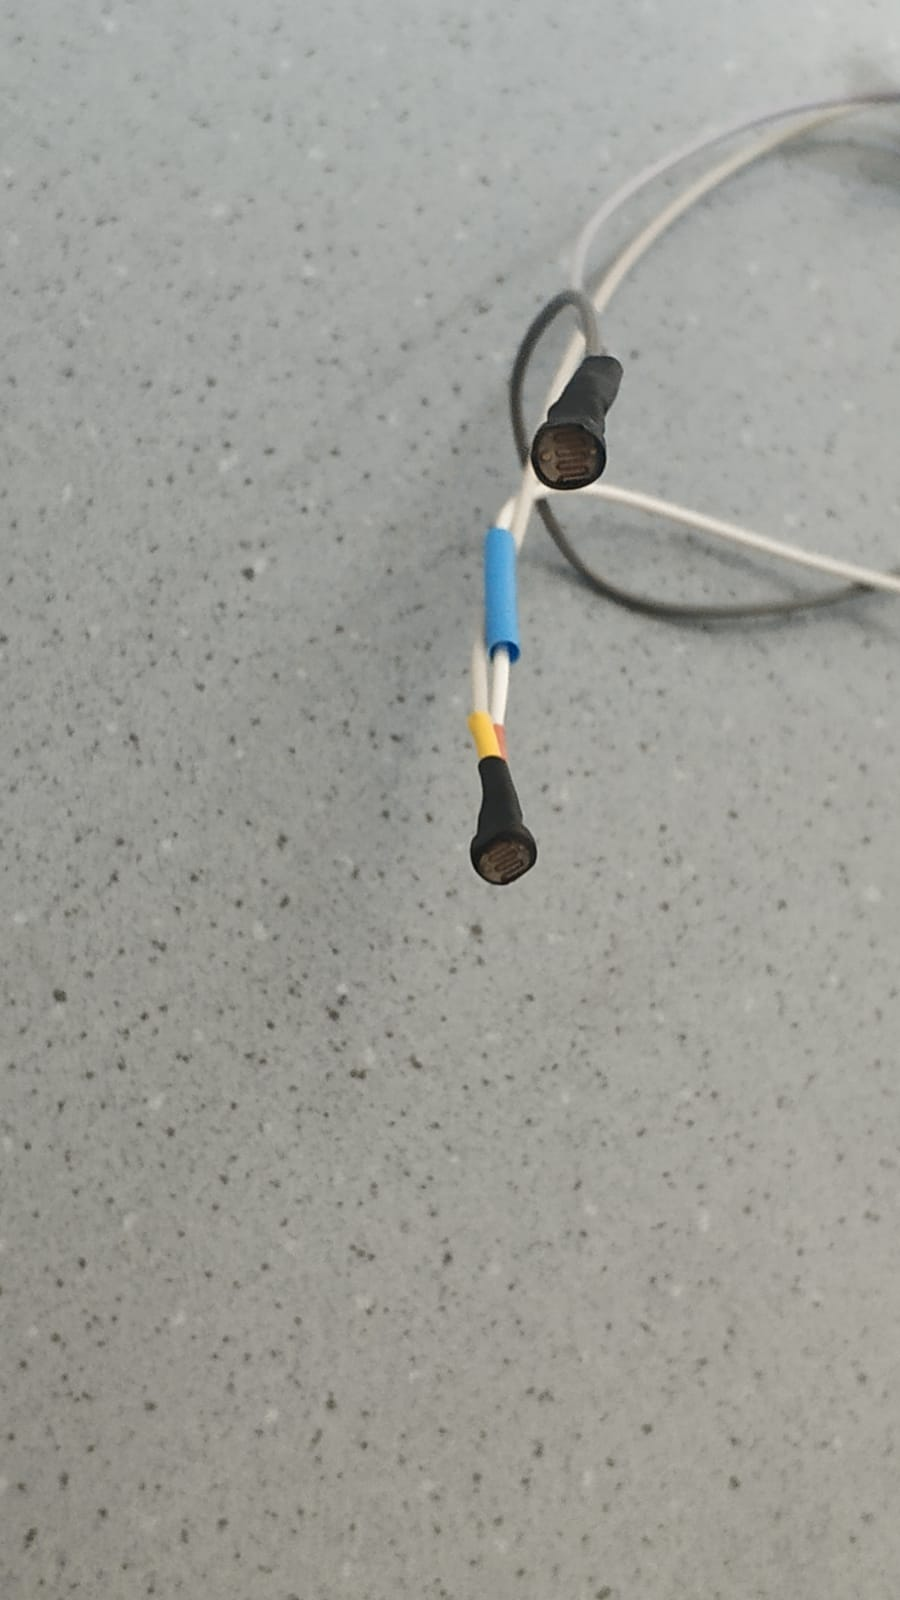
\includegraphics[angle=90, width=\textwidth]{image2x} % Replace with 
    \end{subfigure}
    \hfill
    % Second figure
    \begin{subfigure}{0.45\textwidth}
        \centering
        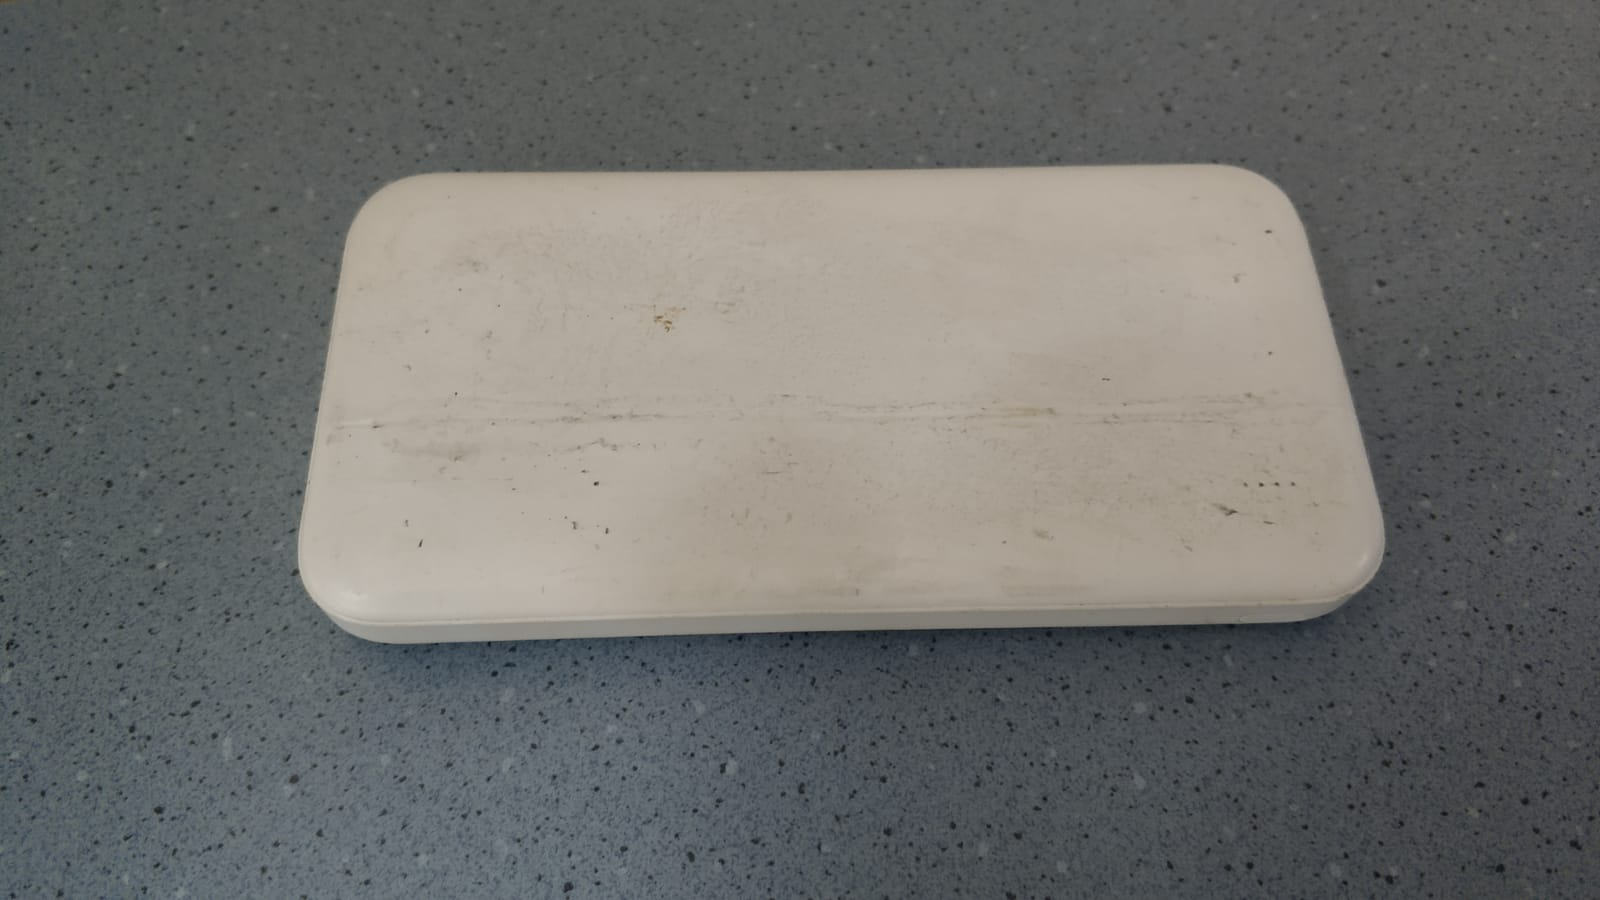
\includegraphics[width=\textwidth]{image1x} % Replace with your file name
    \end{subfigure}
    \caption{Harici Güç Kaynağı ve LDR Sensörü}
    \label{fig:pow_ldr}
\end{figure}

\subsubsection{NUCLEO-STMH723ZG}
Projede merkezi kontrol birimi olarak STM32H723ZG mikrodenetleyicisi tercih edilmiştir. Bu tercih, sistemin yüksek hesaplama gücüne olan ihtiyacı, çoklu sensör birimlerinden gelen verilerin işlenmesi, yapay zeka modeli çalıştırma gereksinimi ve geniş çevresel bağlantı desteği gibi kriterler göz önünde bulundurularak yapılmıştır. 

STM32H723ZG, STMicroelectronics tarafından geliştirilen ve ARM Cortex-M7 çekirdeğini temel alan yüksek performanslı bir mikrodenetleyicidir. 550 MHz saat frekansı, 1 MB flash belleği ve 564 KB RAM kapasitesiyle gömülü sistemlerde ileri düzey işlem yetenekleri sunar. Ayrıca bünyesinde barındırdığı 16-bit çözünürlüğe sahip ADC birimi, LDR sensörlerinden gelen analog sinyallerin hassas bir şekilde dijital verilere dönüştürülmesini mümkün kılmaktadır. UART, SPI, I2C, CAN ve USB gibi çok sayıda haberleşme birimi sayesinde modüler donanım bileşenleriyle kolay entegrasyon sağlanabilmektedir.  

STM32H7 serisi, CMSIS-NN ve TensorFlow Lite for Microcontrollers gibi kütüphanelerle uyumlu çalışarak, sistemde geliştirilen basit sınıflandırma algoritmalarının mikrodenetleyici üzerinde çalıştırılmasına imkân tanımaktadır. Bu sayede sensör verileri yalnızca toplanmakla kalmayıp, aynı zamanda mikrodenetleyici tarafından gerçek zamanlı olarak işlenip karar verici mekanizmalara dönüştürülebilmektedir.

\begin{figure}
    \centering
    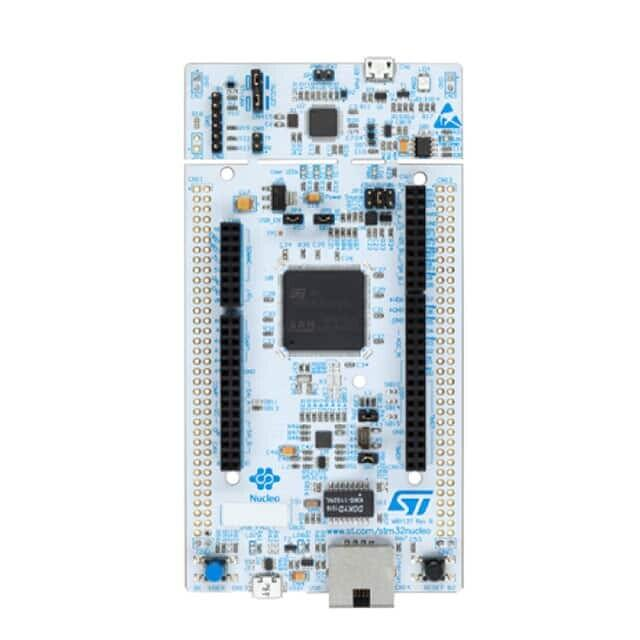
\includegraphics[angle=90, width=0.45\linewidth]{image5x}
    \caption{NUCLEO-STMH723ZG}
    \label{fig:nucleo}
\end{figure}

\subsection{Uygulanan Yöntemler}


\subsubsection{Analog Değerlerin Dijitale Dönüşümü}

Dijital sistemlerde analog sinyallerin işlenebilmesi için ADC (Analog-Dijital Dönüştürücü) devreleri kullanılır. Bu projede, başlangıçta veri toplama ve model oluşturma sürecinde MSP430 mikrodenetleyicisinin dahili 12 bit SAR (Successive Approximation Register) ADC birimi kullanılmıştır. Analog-dijital dönüştürme işlemi, belirli bir gerilim aralığını seçilen ADC çözünürlüğüne göre ölçeklendirerek analog sinyalleri dijital değerlere dönüştürmeyi sağlar. Bu sayede, LDR sensörlerinden elde edilen gerilim değerleri, mikrodenetleyici tarafından işlenebilecek sayısal verilere dönüştürülmüştür. Model oluşturma süreci tamamlandıktan sonra, sistemin daha yüksek çözünürlükte ve daha hızlı karar verebilmesi amacıyla STM32H723ZG mikrodenetleyicisine geçilmiştir. STM32H723ZG'nin bünyesinde bulunan 16 bit ADC modülü sayesinde, LDR sensörlerinden gelen analog veriler daha hassas bir şekilde dijital değerlere dönüştürülmekte ve oluşturulan model doğrultusunda sistemin karar mekanizması çalıştırılmaktadır.

\subsubsection{Bluetooth 2.0 İletişim Protokolü}

Bluetooth bir kısa mesafe iletişim protokolüdür. Projede sensörlerden gelen gerilim verilerinin bilgisayara aktarımını sağlayan teknolojidir. Bluetooth kısa mesafelerde, düşük güçlerde veri aktarımı sağlamak amacıyla tasarlanmış bir protokoldür.

\subsubsection{Üstel Hareketli Ortalama (EMA) Filtreleme}

Üstel Hareketli Ortalama filtreleme zaman serisi verilerindeki gürültüyü azaltmak ve daha pürüzsüz bir sinyal elde etmek için kullanılan bir tekniktir. EMA son verilerin etkisini artırarak hızlı değişimleri daha iyi takip eder.

\subsection{Yazılımlar}

\subsubsection{MSP430 Üzerinde Çalışan Gömülü Yazılım}
Projede MSP430 işlemcisinin belleği üzerine yazılan kaynak kodları LDR sensörler üzerine düşen gerilimlerin takibi amacıyla yazılmıştır. Kodlar ANSI C dilinde yazılmış ve MSP430 işlemcisi için uygun olan CCS derleyicisiyle derlenmiştir. Gömülü kodu yazmak için öğrenciler KTÜ Elektrik-Elektronik Mühendisliği bölümü içerisinde verilen ELK2021 Mikroişlemciler dersinden olan birikimlerini kullanmanın yanı sıra Mikroişlemcinin üretici firması olan Texas Instruments şirketinin işlemciler için sunduğu resmi dökümanlardan faydalanmıştır.

\subsubsection{STM32H723ZG Üzerinde Çalışan Gömülü Yazılım}
Projede STM32H723ZG işlemcisinin belleği üzerine yazılan kaynak kodlar, yapay zeka modelinin işlemci üzerinde çalıştırılması amacıyla geliştirilmiştir. Kodlar C dilinde yazılmış ve STM32H7 serisi için uygun olan STM32CubeIDE ortamında derlenmiştir. Gömülü yazılımı oluşturmak için öğrenciler, KTÜ Elektrik-Elektronik Mühendisliği bölümü kapsamında aldıkları gömülü sistemler ve mikrodenetleyiciler derslerindeki bilgilerini kullanmış; ayrıca işlemci üreticisi STMicroelectronics'in sağladığı referans manüellerden ve yazılım kütüphanelerinden yararlanmıştır.

\subsubsection{Python Yazılım Dili}
Python programlama dili, LDR sensör verilerini Bluetooth aracılığıyla bilgisayara aktarmak için tercih edilmiştir. Bu seçimin temel nedenleri, serial kütüphanesinin veri iletimini kolaylaştırması ve NumPy ile pandas gibi kütüphanelerin verileri CSV formatına dönüştürerek yapay zeka eğitimi için MATLAB'e hazırlanmasını sağlamasıdır. Ayrıca, PyQtGraph gibi kütüphaneler de verilerin görsel olarak izlenmesinde kolaylık sunar.

\subsubsection{MATLAB Yazılım Dili}
Bu çalışmada, yapay zeka modelinin eğitimi için MATLAB yazılımı kullanılmıştır. MATLAB, geniş kapsamlı matematiksel ve mühendislik hesaplamaları destekleyen güçlü bir yazılım ortamı sunmaktadır. Model eğitimi sürecinde, MATLAB'ın Deep Learning Toolbox'ı kullanılarak yapay sinir ağı tasarlanmış ve eğitilmiştir. \ref{fig:yaz}de yazılımların akış şeması görülmektedir.

Mikrodenetleyici, LDR verilerini SAR ADC ile dijitale çevirip Bluetooth ile bilgisayara iletir. Python kodu, dijital LDR verilerini voltaja dönüştürür, EMA filtresi ve geri yönlü sonlu fark yöntemiyle işleyerek, önünden geçen kişiye ait verileri CSV dosyasına kaydeder. Matlab kodu CSV dosyasındaki verileri okuyup veriden özellikleri çıkarır, yapay zeka modelini belirler ve yapay zekayı eğitir.



\subsection{Malzeme Listesi ve Ekonomik Analiz}


\begin{table}[H]
\captionsetup{justification=raggedright, singlelinecheck=false}
\centering
\caption{Malzeme Listesi}
\begin{spreadtab}{{tabular}{|p{3cm}|p{6cm}|p{3cm}|p{1cm}|p{2cm}|}}
\hline
@ Malzemenin Adı                      & @ Kullanım Amacı  & @ Birim fiyatı (TL) & @ Adedi  & @ Fiyatı (TL)       \\ \hline
@ MSP430F5529LP                       & @ Verimli çalışması, 12-bit ADC, Bluetooth modülü entegrasyonu.      & 586.73              & 1        & 586.73              \\ \hline
@ NUCLEO-STMH723ZG                       & @ STM32H723ZG, yüksek performans (550 MHz), geniş bellek ve çoklu haberleşme desteğiyle sensör verilerini işleyip yapay zeka modellerini çalıştırabilir. 16-bit ADC ve AI uyumluluğu sayesinde gerçek zamanlı karar almayı sağlar.      & 1659.95              & 1        & 1659.95             \\ \hline
@ HC05 Seri Bluetooth Modülü          & @ 3.3V besleme seviyesinde çalışması, Bluetooth 2.0 + EDR protokolü ile çalışması,                  & 187.79              & 1        & 187.79              \\ \hline
@ LDR                                 & @ Işığa duyarlı olması sebebiyle voltaj bölücü olarak kullanarak veri çıkarmamız.                  & 6.61                   & 2        & 13.22                   \\ \hline
@ S-link IP-G10N Powerbank            & @ MSP430'u beslemesi, şebeke kesintileri esnasında sistemin devre dışı kalmasını engellemesi ve uzun çalışma süresi olması.                   & 404.91              & 1        & 404.91              \\ \hline
@ Kutu           & @ Kutunun boyutları, bileşenlerin yerleşimi ve işlevselliği için optimize edilmiştir; havalandırma delikleri ve sensör yuvaları, aşırı ısınmayı engelleyerek etkin çalışmayı sağlar.        & 200              & 1        & 200              \\ \hline
\multicolumn{4}{|l|}{@ Toplam} & sum(e2:e7) \\ \hline
\end{spreadtab}
\end{table}

\begin{figure}[H]
    \centering
    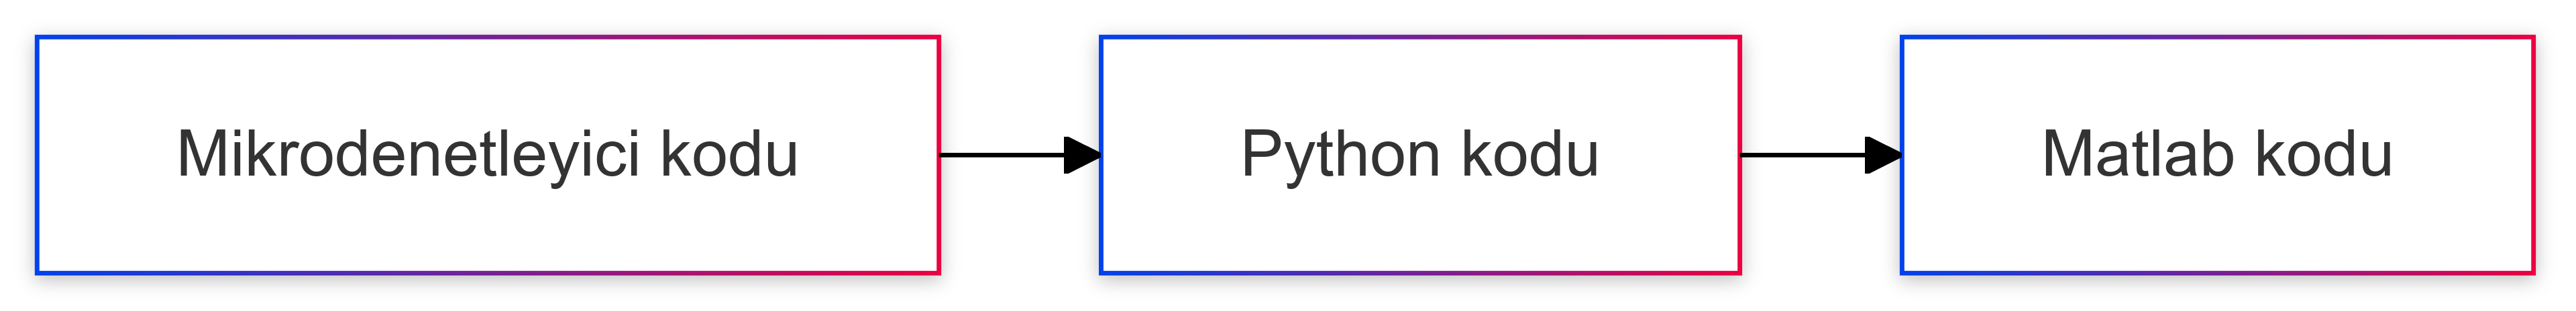
\includegraphics[width=\linewidth]{image13_1}
    \caption{Yazılım Akış Şeması}
    \label{fig:yaz}
\end{figure}

\subsection{Hukuki Boyut}
Bir projenin gerçekleştirilmesi sırasında, çeşitli hukuki sorunlarla karşılaşılabilir.

Fikri Mülkiyet Hakları: Projenin içeriğinde kullanılan yazılım, tasarım, marka veya patentler gibi fikri mülkiyet haklarının ihlali durumlarıdır. Bu, projede kullanılan materyallerin izinsiz kullanılması veya başka bir tarafından sahip olunan fikri mülkiyet haklarının ihlali anlamına gelir.

Veri Güvenliği ve Gizlilik: Projede kullanılan verilerin güvenliği ve gizliliği ile ilgili sorunlar. Özellikle kişisel verilerin korunması gerekiyorsa, bu konuda ihlaller hukuki sorunlara yol açabilir.

Hukuki süreçlerin doğru yönetilmesi, projenin başarıya ulaşmasında kritik bir rol oynayabilir.

\subsubsection{Kişisel Verileri Koruma Kanunu}

Madde 1- (1) Bu Kanunun amacı, kişisel verilerin işlenmesinde başta özel hayatın gizliliği
olmak üzere kişilerin temel hak ve özgürlüklerini korumak ve kişisel verileri işleyen gerçek ve
tüzel kişilerin yükümlülükleri ile uyacakları usul ve esasları düzenlemektir.

Madde 2- (1) Bu Kanun hükümleri, kişisel verileri işlenen gerçek kişiler ile bu verileri
tamamen veya kısmen otomatik olan ya da herhangi bir veri kayıt sisteminin parçası olmak
kaydıyla otomatik olmayan yollarla işleyen gerçek ve tüzel kişiler hakkında uygulanır.

\subsubsection{Teknoloji Geliştirme Bölge Kanunu}

Madde 1 – Bu Kanunun amacı, üniversiteler, araştırma kurum ve kuruluşları ile üretim
sektörlerinin işbirliği sağlanarak, ülke sanayisinin uluslararası rekabet edebilir ve ihracata yönelik bir yapıya kavuşturulması maksadıyla teknolojik bilgi üretmek, üründe ve üretim yöntemlerinde yenilik geliştirmek, ürün kalitesini veya standardını yükseltmek, verimliliği artırmak, üretim maliyetlerini düşürmek, teknolojik bilgiyi ticarileştirmek, teknoloji yoğun üretim ve girişimciliği desteklemek, küçük ve orta ölçekli işletmelerin yeni ve ileri teknolojilere uyumunu sağlamak, (...)\textsuperscript{\cite{kanun7263}} teknoloji yoğun alanlarda yatırım olanakları yaratmak, araştırmacı ve vasıflı kişilere iş
imkânı yaratmak, teknoloji transferine yardımcı olmak ve yüksek/ileri teknoloji sağlayacak yabancı sermayenin ülkeye girişini hızlandıracak teknolojik alt yapıyı sağlamaktır.

b) Teknoloji Geliştirme Bölgesi (Bölge): Yüksek/ileri teknoloji kullanan ya da yeni teknolojilere yönelik firmaların, belirli bir üniversite veya yüksek teknoloji enstitüsü ya da Ar-Ge merkez veya enstitüsünün olanaklarından yararlanarak teknoloji veya yazılım ürettikleri/geliştirdikleri, teknolojik bir buluşu ticari bir ürün, yöntem veya hizmet haline dönüştürmek için faaliyet gösterdikleri ve bu yolla bölgenin kalkınmasına katkıda bulundukları, aynı üniversite, yüksek teknoloji enstitüsü ya da Ar-Ge merkez veya enstitüsü alanı içinde veya yakınında; akademik, ekonomik ve sosyal yapının bütünleştiği siteyi veya bu özelliklere sahip teknoparkı, (...)\textsuperscript{\cite{kanun7263}}

\begin{comment}
Tasarım kısmında, çalışmada yapılan hesaplamalar ilgili teori ve
teoremlere dayandırılarak açıklanmak zorundadır. Yapılacak projenin
teorik altyapısına da bağlı olarak gerekli hesaplamalar ve varsa
çizimler yapılmalıdır. Hesaplamalarda kullanılan sayısal değerler
çizelgeler halinde verilmeli, hesaplama sonuçları da ya çizelge ya da
şekillerle gösterilmelidir. Tasarım çizimlerinde çizim kağıdında başlık
(antet) bulunmalı, çizimin ne zaman, kim ve kimler tarafından, kimin
danışmanlığında, hangi proje kapsamında yapıldığı bilgileri yer
almalıdır. Tasarım çizimlerinda tüm boyutlandırma ölçülerinin sayısal
olarak verilmesi zorunludur. Tasarım bölümünün sonunda yapılacak
çalışmanın tüm detayları ortaya konmalı kullanılacak ve satın alınacak
malzeme listesi çıkarılarak listelenmeli ve \textbf{ön maliyet
hesabı yapılmalıdır.} Ayrıca projenin gerçekleştirilmesi ve sonrasında
kullanılırken oluşturabileceği hukuksal sorunlar araştırılmalı ve
yazılmalıdır.

Tasarımla ilgili bölümler aşağıdaki alt başlıklara sahip olabilir.

---
config:
  layout: fixed
  fontSize: 22px
---
flowchart LR
    A["Harici Batarya"] --> B["Mikrodenetleyici"]
    C["LDR Sensörleri"] --> B
    B --> D["Bluetooth Modülü"]
    D -.-> F["Bilgisayar"]

---
config:
  layout: fixed
  fontSize: 22px
---
flowchart LR
    A["Mikrodenetleyici, LDR verilerini SAR ADC ile dijitale çevirip Bluetooth ile bilgisayara iletir."] --> B["Python kodu, dijital LDR verilerini voltaja dönüştürür, EMA filtresi ve geri yönlü sonlu fark yöntemiyle işleyerek, önünden geçen kişiye ait verileri CSV dosyasına kaydeder."]
    B --> C["Matlab kodu CSV dosyasındaki verileri okuyup veriden özellikleri çıkarır, yapay zeka modelini belirler ve yapay zekayı eğitir."]
    A@{ shape: rect}

\textbf{3.2. Boyutlandırmalar}

Kullanılacak olan masa, kutu, montaj yatağı vb. malzeme
boyutlandırmaları yapılır. İçlerine konulacak elemanların boyutları ve
ara boşlukları da dikkate alınarak kullanılacak dış kutu ve montaj
yatağı gibi kısımlar boyutlandırılır.

\textbf{3.3. Sistem Bileşenleri ve Seçimleri}

Kullanılacak olan alt sistem bileşenlerinin neler olduğu ve nasıl
seçildikleri bu ayrıtta açıklanabilir. Seçilen komponentlerin
fotograflarını vermek onların açıklanması anlamına gelmez. Unutulmamalı
ki bu yazılan rapor bir Tasarım Projesi Raporu veya bir Bitirme Projesi
Tez Kitabıdır. Ürün katoloğu değildir. Kullanılan elemanlar
fotoğraflarıyla değil, teknik özellikleri ve projede neden, nasıl
kullanıldıkları öne çıkarılarak açıklanmalıdırlar. Nasıl seçildikleri de
açıklanmalıdır.

\textbf{3.4. Uygulanan Yöntemler}

Çalışmanın değişik safhalarında uygulanan yöntemler bu ayrıtta
açıklanmalıdır. Devre tasarım yöntemleri, kontrol yöntemleri, sayısal
çözümleme yöntemleri, haberleşme yöntemleri, konuya özgü ne tür uygulama
yöntemi yarsa burada açıklanmalıdır.

\textbf{3.5. Yazılımlar}

Çalışmada yazılım geliştirilmişse bu yazılıma ait akış şeması burada
verilerek gerekli açıklamalar yapılmalıdır. Yazılımın kodunu burada
vermeyiniz. Eğer tez danışmanı öğretim üyesi yazılım kodunun mutlaka
konulmasını isterse o zaman ekler kısmına ayrı bir ek olarak
eklenebilir.

Çalışmanın simülasyonu için kullanılan paket program türü yazılım varsa
o yazılımdan da burada kısaca bahsedilebilir. Sümülasyon çalışmasını
burada anlatmayınız. Bir sonraki bölüm zaten doğrudan simülasyon
çalışmaları içindir.

\newpage

\textbf{3.6. Malzeme Listesi ve Ekonomik Analiz}

Çalışmada kullanılacak olan malzemelerin tam listesi bu ayrıtta verilir.
Çizelge 3.1 dekine benzer bir çizelge halinde malzemenin ismi, nerede
niçin kullanılacağı, birim fiyatı ve kaç addet gerektiği yazılır. Tüm
malzemelerin fiyatları toplanarak genel bütçe oluşturulur ve proje
bütçesi ile karşılaştırılır. Bütçeye uygun bir malzeme listesi
oluşturmak için ne tür değerlendirmeler ve tercihler yapıldığı da burada
açıklanır. Kullanılacak malzemelerin fiyat ve kalitesinin proje
üzerindeki olumlu ve olumsuz etkileri değerlendirilerek buraya yazılır.

Çizelge 3.1. Malzeme Listesi

\begin{longtable}[l]{@{}
  >{\raggedright\arraybackslash}p{(\columnwidth - 8\tabcolsep) * \real{0.2585}}
  >{\raggedright\arraybackslash}p{(\columnwidth - 8\tabcolsep) * \real{0.2951}}
  >{\raggedright\arraybackslash}p{(\columnwidth - 8\tabcolsep) * \real{0.1968}}
  >{\raggedright\arraybackslash}p{(\columnwidth - 8\tabcolsep) * \real{0.0984}}
  >{\raggedright\arraybackslash}p{(\columnwidth - 8\tabcolsep) * \real{0.1512}}@{}}
\begin{tabular}{|llll|l|}
\hline
\multicolumn{1}{|l|}{Malzemenin adı} & \multicolumn{1}{l|}{Kullanım amacı} & \multicolumn{1}{l|}{Birim fiyatı (TL)} & Adedi & Fiyatı (TL) \\ \hline
\multicolumn{1}{|l|}{}               & \multicolumn{1}{l|}{}               & \multicolumn{1}{l|}{}                  &       &             \\ \hline
\multicolumn{1}{|l|}{}               & \multicolumn{1}{l|}{}               & \multicolumn{1}{l|}{}                  &       &             \\ \hline
\multicolumn{1}{|l|}{}               & \multicolumn{1}{l|}{}               & \multicolumn{1}{l|}{}                  &       &             \\ \hline
\multicolumn{1}{|l|}{}               & \multicolumn{1}{l|}{}               & \multicolumn{1}{l|}{}                  &       &             \\ \hline
\multicolumn{4}{|r|}{TOPLAM}                                                                                                &             \\ \hline
\end{tabular}
\end{longtable}

\textbf{3.7. Hukuki Boyut}

Projenin konusuna bağlı olarak gerçekleştirilmesi sırasında
karşılaşılabilecek hukuki sorunlar bu başlık altında
değerlendirilmelidir. Proje tamamlandıktan sonra karşılaşılabilecek
hukuki sorunlara da burada yer verilmelidir. Proje konusu ile ilgili
yönetmeliklere ve mevzuatlara de burada yer verilir. Bu konuda
\textbf{mevzuat.gov.tr} web adresi faydalı olabilir.
\end{comment}


\begin{comment}

Yeni işlemciye geçildi. Yeni işlemcinin bağlantıları farklı olucak o yüzden bağlantı yeni bağlantı şeması lazım. boyutu farklı bu yüzden kutu tasarımı değişecek. 



\end{comment}
